Целью данной работы стало исследование почтового клиента Mozilla Thunderbird, написание программного модуля для сбора сообщений и представления их в формате XML.

\subsubsection{Реализация программного модуля}

В ходе изучения приложения было выяснено расположение файлов, хранящих почтовые сообщения. Эти данные представлены в таблице~\ref{tab:data}, где:

\begin{itemize}
  \item profile\_name --- может быть любым и генерируется самой программой (например, g5bq66yo.default);
  \item server\_name --- название сервера входящей почты (например, imap.yandex.com).
\end{itemize}

\begin{table}[ht]
\caption{Местоположение и название файлов}
\label{tab:data}
\begin{center}
\begin{tabularx}{\linewidth}{|X|X|X|X|}
\hline
Протокол & Путь & Файл с входящими сообщениями & Файл с исходящими сообщениями \\
\hline
imap & C:\textbackslash Users\textbackslash User\textbackslash AppData   & INBOX & \textampersand BB4EQgQ,BEAEMAQ\\
     & \textbackslash Roaming\textbackslash Thunderbird                  &       & yBDsENQQ9BD0ES \\
     & \textbackslash Profiles\textbackslash profile\_name  &   & wQ1- \\
     & \textbackslash ImapMail\textbackslash server\_name   &   &      \\
\hline
pop3 & C:\textbackslash Users\textbackslash User\textbackslash AppData & Inbox & Sent \\
     & \textbackslash Roaming\textbackslash Thunderbird                &       &      \\
     & \textbackslash Profiles\textbackslash profile\_name             &       &      \\
     & \textbackslash Mail\textbackslash server\_name                  &       &      \\
\hline
\end{tabularx}
\end{center}
\end{table}

Для каждого почтового аккаунта, который подключен в Thunderbird, создается своя папка <<server\_name>>. Данные указаны для windows 7, 8, 8.1.

Проводник Windows не может определить расширение файлов, но при открытии любым текстовым редактором можно понять, что файлы имеют формат mbox. Mbox представляет собой текстовый файл, в котором хранятся все сообщения почтового ящика. Начало почтового сообщения определяется строкой из 5 символов: словом <<From>> с последующим пробелом.

Пример сообщения:

\begin{verbatim}
  From 
  Message-ID: <55600F73.6020804@yandex.ru>
  Date: Sat, 23 May 2015 11:26:11 +0600
  From: fgfgsr <art0rias@yandex.ru>
  User-Agent: Mozilla/5.0 (Windows NT 6.1; WOW64; rv:31.0) 
              Gecko/20100101 Thunderbird/31.7.0
  MIME-Version: 1.0
  To: yuriy94@hotmail.com
  Content-Type: text/plain; charset=utf-8; format=flowed
  Content-Transfer-Encoding: 7bit

  Little girl, little girl, Where have you been?
\end{verbatim}

В блоке с сообщением хранятся данные о дате, отправителе, получателе, версии почтового клиента, является ли письмо ответом на другое, а также заголовок и текст письма.

\subsubsection{Алгоритм работы модуля}

После открытия файл mbox разделяется на отдельные сообщения с помощью регулярного выражения <<(From \textbackslash \textbackslash r\textbackslash \textbackslash n)|(From \textbackslash \textbackslash n\textbackslash \textbackslash r)|From \textbackslash \textbackslash r|From \textbackslash \textbackslash n>>. Затем к каждому сообщению применяются регулярные выражения:

\begin{itemize}
  \item <<\textbackslash \textbackslash nDate: ([\textasciicircum \textbackslash \textbackslash n]*)\textbackslash \textbackslash n>> --- время отправки/приема сообщения;
  
  \item <<\textbackslash \textbackslash nFrom: .*([a-z][\textbackslash \textbackslash w\textbackslash \textbackslash .]*\textbackslash \textbackslash w@\textbackslash \textbackslash w[\textbackslash \textbackslash w\textbackslash \textbackslash .]*\textbackslash \textbackslash .\textbackslash \textbackslash w*).*\textbackslash \textbackslash nUser-Agent:>> --- кто отправил сообщения;
  
  \item <<\textbackslash \textbackslash nTo: .*([a-z][\textbackslash \textbackslash w\textbackslash \textbackslash .]*\textbackslash \textbackslash w@\textbackslash \textbackslash w[\textbackslash \textbackslash w\textbackslash \textbackslash .]*\textbackslash \textbackslash .\textbackslash \textbackslash w*).*\textbackslash \textbackslash nSubject:>> --- кто получил сообщение;
  
  \item <<\textbackslash \textbackslash nContent-Transfer-Encoding: 8bit\textbackslash \textbackslash s*(\textbackslash \textbackslash S.*\textbackslash \textbackslash S)\textbackslash \textbackslash s*[0-3]\textbackslash \textbackslash d\textbackslash \textbackslash .[01]\textbackslash \textbackslash d\textbackslash \textbackslash .\textbackslash \textbackslash d{4} [0-2]\textbackslash \textbackslash d:[0-5]\textbackslash \textbackslash d, [\textasciicircum \textbackslash \textbackslash n]*\textbackslash \textbackslash n>> --- текст сообщения.
\end{itemize}

Блок-схема алгоритма представлена на рисунке~\ref{teresh_1:teresh_1}.

\begin{figure}[h!]
\center{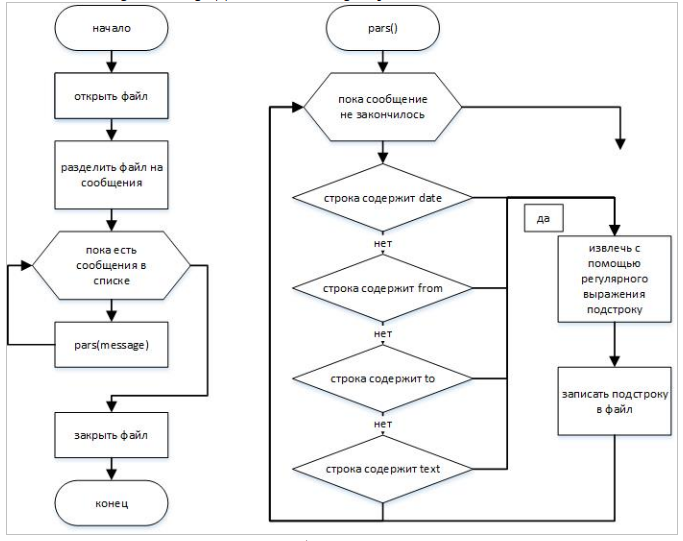
\includegraphics[width=0.9\linewidth]{teresh_1}}
\caption{Блок-схема алгоритма}
\label{teresh_1:teresh_1}
\end{figure}

\clearpage

\subsubsection{Структура XML-файла}

Документы XML имеют иерархическую структуру и начинаются с элемента <add> --- это начальный элемент документа (корень). Далее будут записаны n дочерних элементов <file>, где n --- количество файлов mbox. В каждый элемент <file> будут записаны m дочерних элементов <message>, где m --- количество сообщений в одном файле, в теле которых будет записано нужное нам количество полей для записи информации. В последнюю очередь записывается конечный элемент </add>.

Пример файла message\_report.xml приведен на рисунке~\ref{teresh_2:teresh_2}.

Значения полей date, from, to, text содержат время и дату, отправителя, получателя, текст сообщения соответственно. Поле name содержит полный путь к mbox файлу.

\begin{figure}[h!]
\center{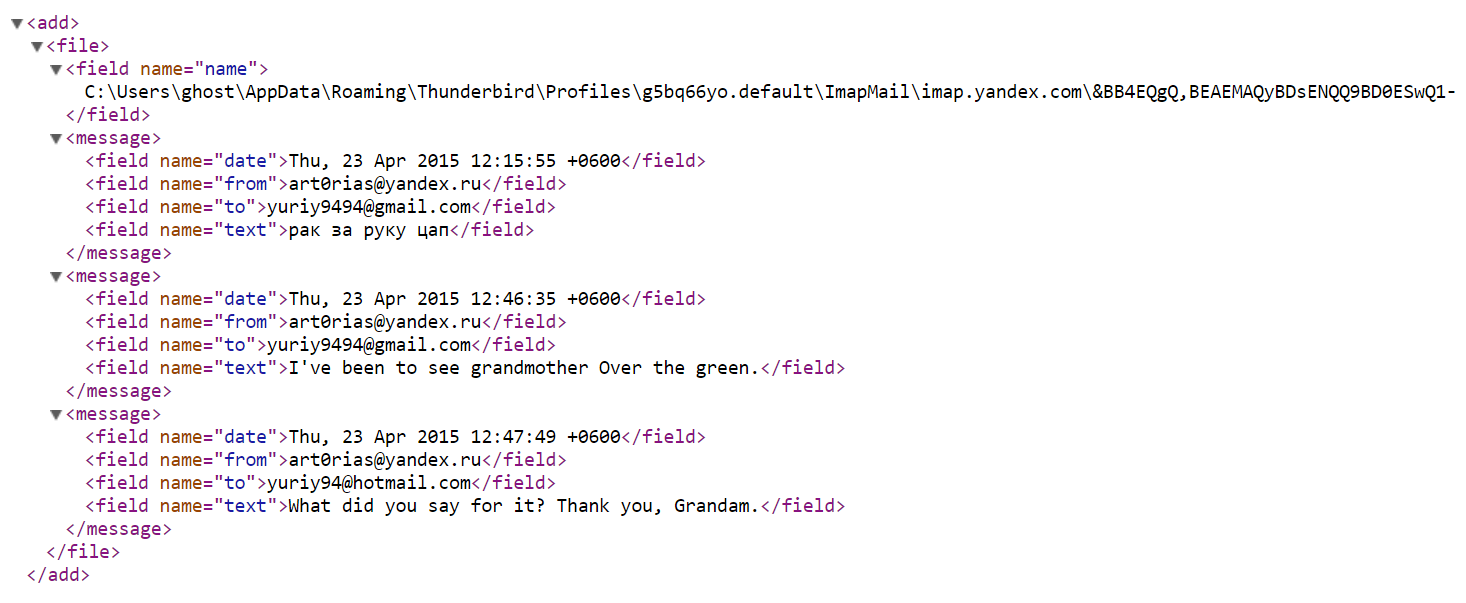
\includegraphics[width=0.9\linewidth]{teresh_2}}
\caption{Пример XML-файла}
\label{teresh_2:teresh_2}
\end{figure}
